\renewcommand{\chaptername}{\scshape Partie}
\chapter{\normalfont \scshape Photographie de l'onde de choc}
\section{Résultats attendus}
D’après la relation \ref{indice_pression} (c.f. Partie 1), un autre moyen de faire varier la masse volumique du milieu est de changer la pression: c’est ce que fait une onde de choc. On fait l’hypothèse que la pression au niveau de l’onde de choc observée est la même que la pression à la rupture de la membrane (\textbf{$P$ = 2,5 bar}), ainsi en utilisant à nouveau la relation des gaz parfait on en déduit une variation d’indice optique très forte  :
\begin{align}
	\rho' - \rho \,&= \,\,\,\frac{M}{R \, T}\,\,(P'-P)
\end{align}
Ce qui donne une variation d'indice de : $\frac{\Delta n}{n} = 39,7\,\%$\\ \\
On s'attend donc à ce que le contraste soit bien visible dans l'image de l'onde de choc. Cependant, vu la grande variation de pression, l'onde de choc se propage à très grande vitesse. En effet, d'après la loi de \textsc{Mach} :
\begin{align}
	c= \sqrt{\gamma\,\frac{P}{\rho}}
\end{align}
Or, \textbf{$\gamma = \frac{7}{5}$}, ce qui donne à peu près \textbf{$c=520\, m/s$} à \textbf{2,5 bar}.
\section{Observations}
\begin{figure}[H]
	\centering
	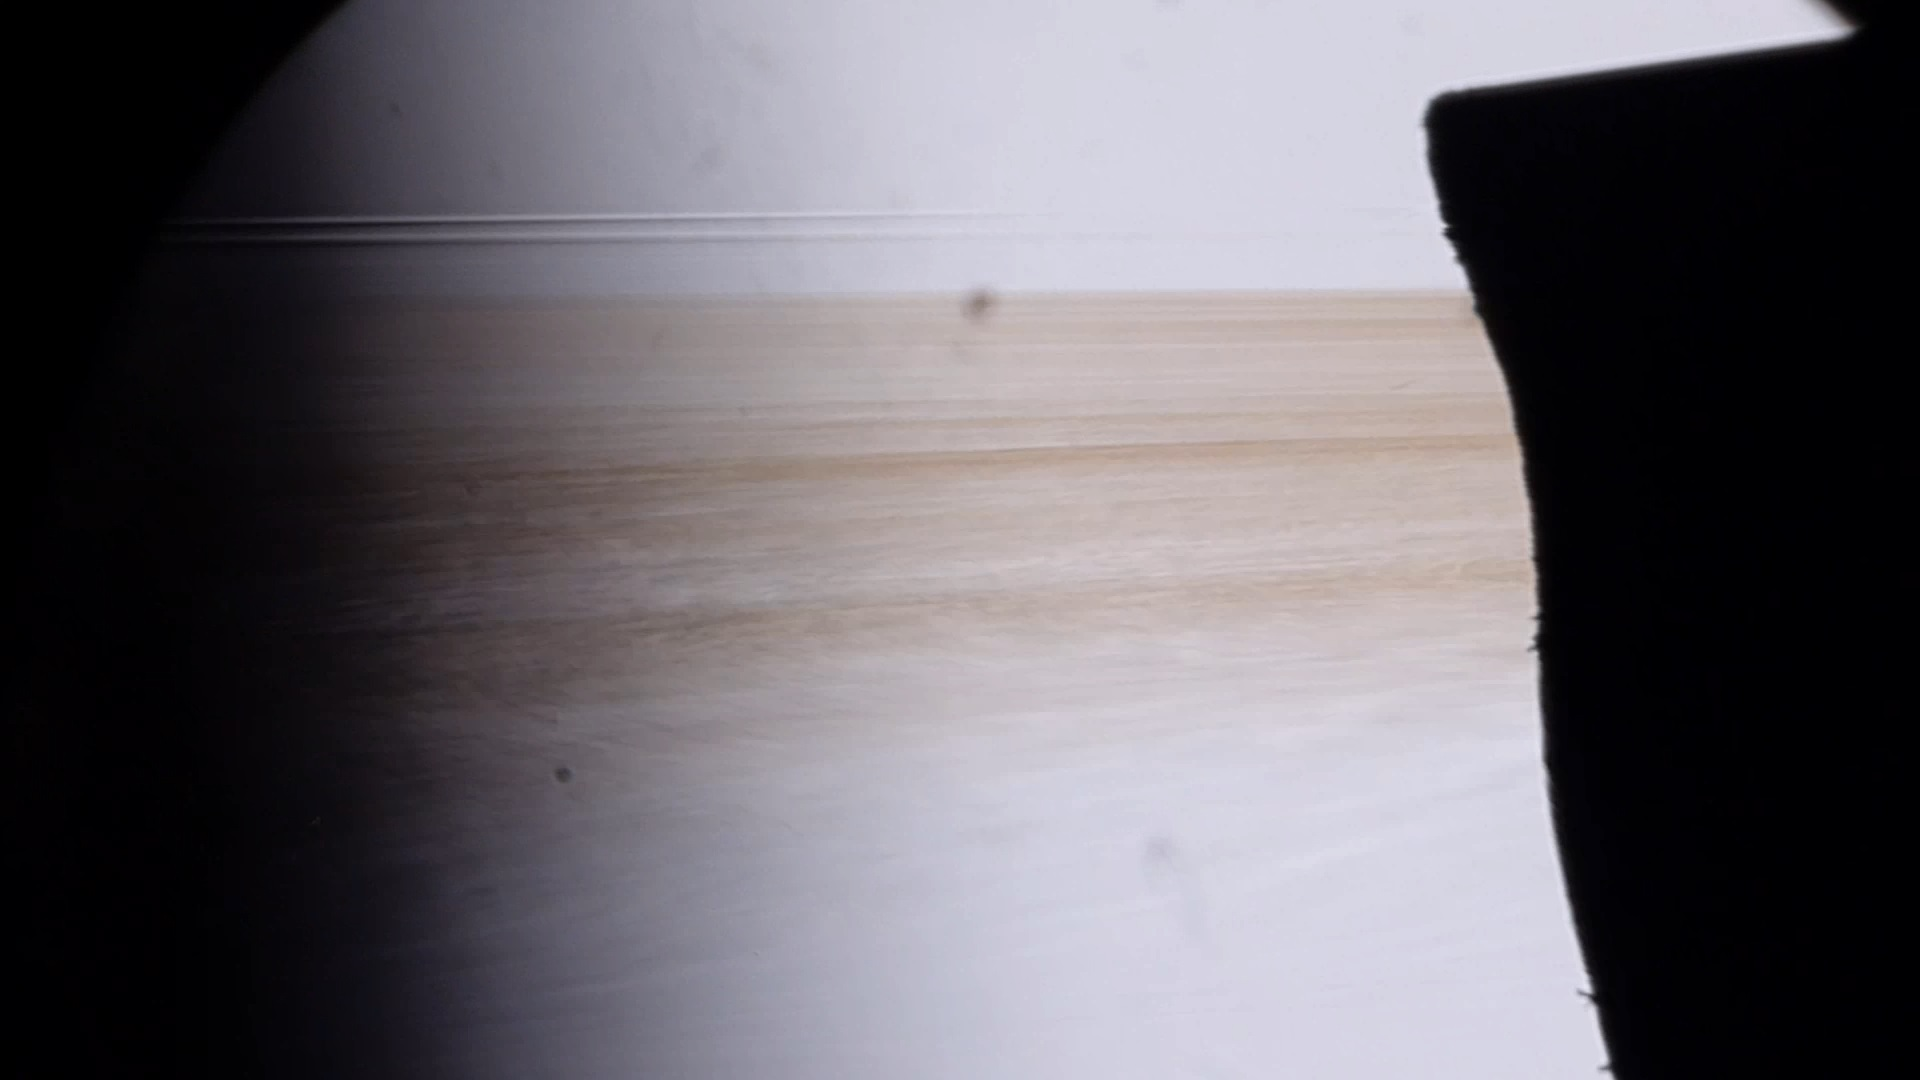
\includegraphics[scale = 0.15]{figures/choc_schlieren.jpg}
	\caption{\small{\textit{Cône de pression lié à l'onde choc, pression avant rupture : 2,5 bars}}}
	\label{choc_schlieren}
\end{figure}